\documentclass[cjk,dvipdfmx,12pt,compress,%
hyperref={bookmarks=true,bookmarksnumbered=true,bookmarksopen=false,%
  colorlinks=false,%
  pdftitle={第 66 回 関西 Debian 勉強会@KOF2012},%
  pdfauthor={佐々木洋平},%
%  pdfinstitute={関西 Debian 勉強会},%
  pdfsubject={資料},%
}]{beamer}
\title{Debian 7.0 ``Wheezy''}
\subtitle{%
  $\sim$第66回関西Debian勉強会@KOF2012$\sim$}
\author{%
  佐々木洋平/Youhei SASAKI \\%
  mailto: \texttt{uwabami@debian.or.jp} \\%
  twitter/IRC nic: \texttt{uwabami} %
}
\institute{%
  {\footnotesize{Debian JP Project/関西 Debian 勉強会}}}
\date{%
  {\footnotesize{2012年11月10日 - 於: 大阪南港ATC 9F room \#3}}}
\usepackage{graphicx}
\usepackage{moreverb}
\usepackage[varg]{txfonts}
\AtBeginDvi{\special{pdf:tounicode EUC-UCS2}}
\usetheme{Kyoto}
% \renewcommand{\familydefault}{\gtdefault}
\renewcommand{\kanjifamilydefault}{\gtdefault}

\begin{document}
\settitleslide
\begin{frame}
  \titlepage
\end{frame}
\setdefaultslide

\takahashi[100]{どーも}
\takahashi[100]{佐々木\\です}

\begin{frame}{About me...}
  \begin{columns}
    \begin{column}{.7\textwidth}
      \begin{itemize}
      \item 佐々木 洋平/ Youhei SASAKI
      \item Twitter / \texttt{@uwabami}
      \item Debian JP Project/関西Debian勉強会
      \item Ruby, TeX, GIS, Scientific Computing, etc...
      \item 普段: 大学で数値計算とか流体力学とか.
      \end{itemize}
    \end{column}
    \begin{column}{.29\textwidth}
      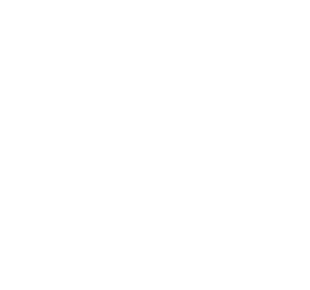
\includegraphics[width=.9\textwidth]{./image201211/face.png}
      \\
      
\includegraphics[width=.9\textwidth]{./image201211/OSC_GPG.png}
    \end{column}
  \end{columns}
\end{frame}

\begin{frame}{Disclaimer}
  \begin{itemize}
  \item 用法, 用量を守って正しくお使い下さい
  \item 誤字脱字含め, 適宜ご指摘下されば幸いです.
  \item 疑問, 質問, ツッコミ, 茶々, \alert{大歓迎}
  \item その場でインタラクティブにどうぞ
\end{itemize}
\end{frame}

\takahashi[40]{今回のお話}
\pgfdeclareimage[width=1.0\paperwidth]{wheezy}{./image201211/non-free/1000px-Wheezy3.jpg}
\settitleslide
\setbeamertemplate{background}{\pgfuseimage{wheezy}}
\begin{frame}\end{frame}
%
\begin{frame}
  \begin{center}
    {\fontsize{80pt}{80pt}\alert{Wheezy}}
  \end{center}
\end{frame}
\setdefaultslide

\begin{frame}[containsverbatim]{Debian 7.0 "Wheezy" is \\ \hspace{5.5ex} now under freeze!!}

  \begin{commandline}

To: debian-devel-announce@lists.debian.org
Subject: 5... 4... 3... 2... 1...
From: "Adam D. Barratt" <adam@adam-barratt.org.uk>
Date: Sat, 30 Jun 2012 21:20:55 +0100

Hi,

As previously announced[1], testing is now frozen.

- snip -

Adam,
for the Debian Release Team

\end{commandline}

\end{frame}

\takahashi[50]{と, いうわけで}

\begin{frame}{Agenda}
  \begin{itemize}
  \item<2-> {\color{red}「フリーズって何?」 \\
      Debian のリリースサイクルについて}
  \item  「で、Wheezyってどうよ?」\\
    Debian 7.0 "Wheezy" の変更点、現状
  \item 「ところで次のリリースは?」\\
    次期リリース Debian 8.0(?) へ向けて
  \end{itemize}
\end{frame}

\section{フリーズって何?}

\takahashi[40]{フリーズって何?}

\takahashi[40]{Debian Infographics}

\pgfdeclareimage[width=1.0\paperwidth]{infographics}{image201209/infographic_debian-ja-v1-1.png}
\settitleslide
\setbeamertemplate{background}{\pgfuseimage{infographics}}
\begin{frame}\end{frame}
\setdefaultslide

\begin{frame}{Debianの\\ \hspace{5.5ex}「ディストリビューション」}

\begin{itemize}
\item 3つの「ディストリビューション」\\
  stable, testing, unstable
\item ディストリビューション以外の「リポジトリ」\\
  updates(旧volatile), security-updates \\
  backports, experimental \\
\end{itemize}

\end{frame}

\takahashi[40]{Debianの\\リリースサイクル}

\pgfdeclareimage[width=1.0\paperwidth]{Cycle01}{image201011/Debian-Release-Cycle01.png}
\pgfdeclareimage[width=1.0\paperwidth]{Cycle02}{image201011/Debian-Release-Cycle02.png}
\pgfdeclareimage[width=1.0\paperwidth]{Cycle03}{image201011/Debian-Release-Cycle03.png}
\pgfdeclareimage[width=1.0\paperwidth]{Cycle04}{image201011/Debian-Release-Cycle04.png}
\pgfdeclareimage[width=1.0\paperwidth]{Cycle05}{image201011/Debian-Release-Cycle05.png}
\settitleslide
\setbeamertemplate{background}{\pgfuseimage{Cycle01}}
\begin{frame}\end{frame}%1
\setbeamertemplate{background}{\pgfuseimage{Cycle02}}
\begin{frame}\end{frame}%2
\setbeamertemplate{background}{\pgfuseimage{Cycle03}}
\begin{frame}\end{frame}%3
\setbeamertemplate{background}{\pgfuseimage{Cycle04}}
\begin{frame}\end{frame}%4
\setbeamertemplate{background}{\pgfuseimage{Cycle05}}
\begin{frame}\end{frame}%5

\takahashi[40]{よくある誤解}


\begin{frame}{今までのリリースサイクル}

\begin{center}
  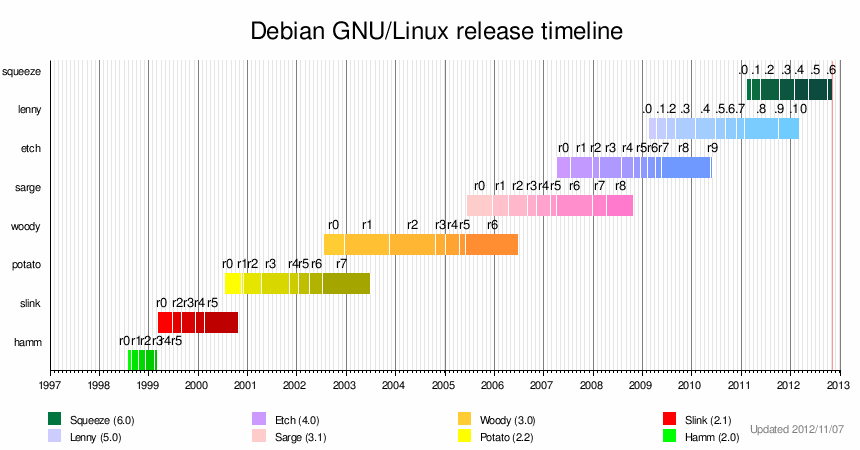
\includegraphics[width=1\textwidth]{image201211/timeline.png}
\end{center}

\end{frame}

\begin{frame}{今までのリリースサイクル}

\begin{itemize}
\item \sout{Debianのリリースは予測不可能/遅れるのが当たり前}
\item \alert{Etch から ほぼ 2 年毎のリリース}
  \begin{itemize}
  \item 3.1 "Sarge"   : 約 3 年
  \item 4.0 "Etch"    : 22ヶ月
  \item 5.0 "Lenny"   : 22ヶ月
  \item 6.0 "Squeeze" : 24ヶ月
  \end{itemize}
\end{itemize}
\end{frame}

\begin{frame}{Time Based Release Freeze}

\begin{center}
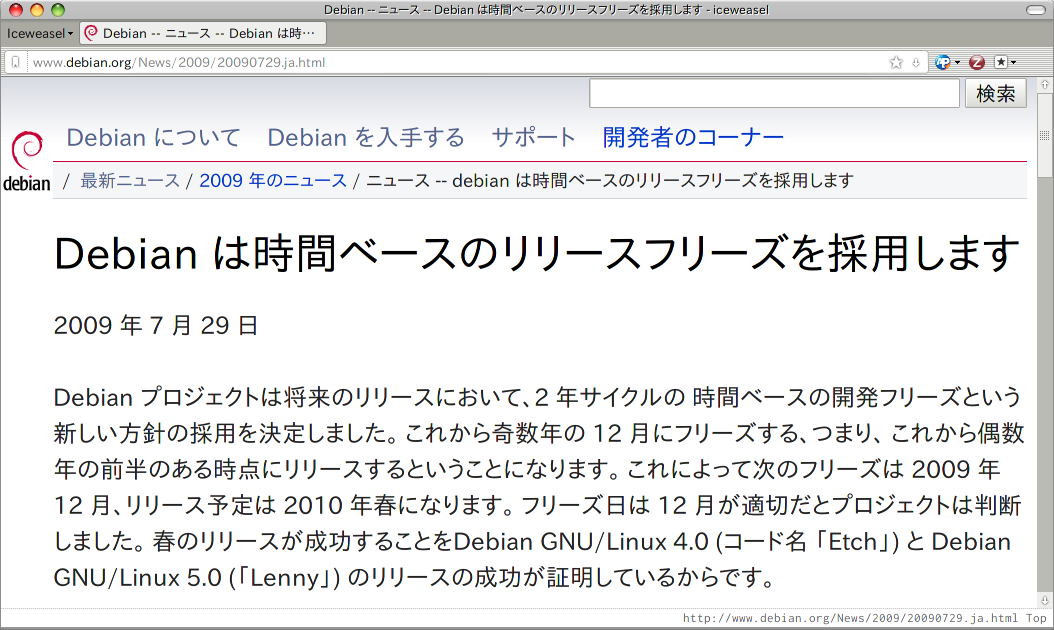
\includegraphics[width=1\hsize]{image201208/Debian_News_2009-07-29-TimeBasedReleaseFreeze.png}
\end{center}

\end{frame}

\begin{frame}{Time Based Release Freeze}

\begin{itemize}
\item testing の フリーズは2年単位になった!!
  \begin{itemize}
    \item Squeeze の Freeze / 2010/08/06 \\$\rightarrow$ 2011/02/06 リリース!
    \item Wheezy の Freeze 2012/06/30 \\$\rightarrow$ 2012/12?
  \end{itemize}
\item 利点:
  \begin{itemize}
    \item 使用者: リリースの時期を予測できる
    \item 開発者: 長期プランを立てやすくなる
  \end{itemize}
\end{itemize}

\end{frame}

\begin{frame}{まとめ: Debian のリリースサイクル}

\begin{itemize}
  \item Debian = 常に進化し続けるディストリビューション
  \begin{itemize}
    \item stable, testing, unstable
    \item 頑健な「stable」と最前線を疾走する「unstable」
  \end{itemize}
  \item Time Based Release Freeze
  \begin{itemize}
    \item \sout{「リリースが遅い/読めない」}→約二年毎の安定版のリリース
    \item 定期的なリリースフリーズによる "huge jump" の回避
  \end{itemize}
\end{itemize}

\end{frame}

\takahashi[40]{Have any\\questions?}

\section{Debian "7.0" Wheezy}
\takahashi[40]{Debian "7.0" Wheezy}
\settitleslide
\setbeamertemplate{background}{\pgfuseimage{wheezy}}
\begin{frame}\end{frame}
\setdefaultslide

% \begin{frame}{Debian "7.0" Wheezy}
%   \begin{itemize}
%   \item \alert{2012/06/30 にフリーズ!!} $\rightarrow$ 現在は{\color{green}{frozen}}
%   \item \alert{リリースに向けたバグ(RCバグ)潰しが進行中}
%   \end{itemize}
% \end{frame}

\settitleslide
\setbeamertemplate{background}{\pgfuseimage{Cycle04}}
\begin{frame}\end{frame}
\begin{frame}
  \begin{center}
    {\fontsize{80pt}{80pt}\selectfont{\alert{いま\\ここ!}}}
  \end{center}
\end{frame}
\settitleslide

\pgfdeclareimage[width=1.0\paperwidth]{RC}{./image201211/non-free/graph.png}
\settitleslide
\setbeamertemplate{background}{\pgfuseimage{RC}}
\begin{frame}\end{frame}
\begin{frame}
  \begin{center}
    {\fontsize{40pt}{40pt}\selectfont 2012/11/10 現在 \\RC バグ: \color{green}{\fbox{\color{black}{455}}}}
  \end{center}
\end{frame}
\setdefaultslide

\takahashi[40]{Wheezyの\\リリースゴール}

\begin{frame}{Wheezy のリリースゴール(1)}
  \begin{itemize}
  \item Multiarch への移行
  \item kFreeBSD (← テクノロジープレビューだった)
  \item IPv6 完全サポート
  \item ラージファイルサポート
  \item .la ファイルの削除
  \end{itemize}
\end{frame}

\begin{frame}{Wheezy のリリースゴール}

\begin{itemize}
  \item {\color{red}Multiarch への移行}
  \item kFreeBSD (← テクノロジープレビューだった)
  \item IPv6 完全サポート
  \item ラージファイルサポート
  \item .la ファイルの削除
\end{itemize}

\end{frame}

\begin{frame}{Multiarch}

\begin{itemize}
  \item 同一のシステム上で、異なるハードウェアアーキテクチャのライブラリ等をインストールする仕組み\\
    \texttt{/usr/lib/} $\rightarrow$ \texttt{/usr/lib/x86\_64-linux-gnu} \\
  \item 何が嬉しいのか?
  \begin{itemize}
    \item 類似のアーキテクチャを一緒に動作させることができる\\
    $\rightarrow$ i386 on amd64, armel on armhf \\
    \item クロスビルド環境の構築が容易になる
  \end{itemize}
\end{itemize}

\end{frame}

\begin{frame}[containsverbatim]{Multiarch: どうやって?}

\begin{commandline}
# dpkg --add-architecture i386
# dpkg --print-foreign-architectures
i386
# echo "deb [arch=i386,amd64] \
  http://ftp.jp.debian.org/debian/ wheezy main" \
   > /etc/apt/sources.list
# apt-get update
# apt-get install libc6:i386
# dpkg --remove-architecture i386
\end{commandline}
%$
%\footnote{\url{http://wiki.debian.org/ReleaseGoals/MultiArch}}

\end{frame}


\begin{frame}{Wheezy のリリースゴール(2)}

  New for Wheezy
  \begin{itemize}
  \item Security hardening build flags
  \item /run への移行
  \item Video4Linux1 を使っているパッケージの修正および削除
  \item /dev/dsp を使っているパッケージの修正および削除
  \end{itemize}

\end{frame}


\begin{frame}{Wheezy のリリースゴール}

New for Wheezy
\begin{itemize}

  \item {\color{red}{Security hardening build flags}}
  \item /run への移行
  \item Video4Linux1 を使っているパッケージの修正および削除
  \item /dev/dsp を使っているパッケージの修正および削除

\end{itemize}

\end{frame}


\begin{frame}{Security hardening build flags}
パッケージ構築時にセキュリティを強化するコンパイルフラグを(デフォルトで)有効にする。

\begin{itemize}
  \item Format string checks( -Wformat -Werror=format-security )\\
  format 使う関数(例えば printf)の使用が問題を引き起こす可能性がある場合に警告する。
  \item FORTIFY\_SOURCE \\
  文字列やメモリの操作を行う関数を使用する際にバッファオーバーフローを検出する。

\end{itemize}

\end{frame}



\begin{frame}{Security hardening build flags}
パッケージ構築時にセキュリティを強化するコンパイルフラグを(デフォルトで)有効にする。

\begin{itemize}
  \item -fstack-protector --param=ssp-buffer-size=4 \\
  スタック破壊攻撃等によるバッファオーバーフローをチェックするための追加コードを生成する。
  4バイトを超える配列を持つ関数を対象にする。
  \item -z,now,-z,relro \\
  リロケーション領域(GOTなど)をリードオンリーにする。
\end{itemize}

\end{frame}


\begin{frame}{Wheezy のリリースゴール}

New for Wheezy
\begin{itemize}

  \item Security hardening build flags
  \item {\color{red}{/run} への移行}
  \item Video4Linux1 を使っているパッケージの修正および削除
  \item /dev/dsp を使っているパッケージの修正および削除

\end{itemize}

\end{frame}


\begin{frame}{/run}

boot の早い段階で一時ディレクトリを用意
\begin{itemize}
  \item /var/run → /run
  \item /var/lock → /run/lock
  \item /dev/shm → /run/shm
  \item /tmp → /run/mp
\end{itemize}

\end{frame}


\takahashi[40]{主なパッケージのバージョン}

\begin{frame}{主なパッケージのバージョン / 1}

\begin{itemize}
  \item Kernel: Linux 3.2, Freebsd 8.3, 9.0
  \item libc: eglibc 2.13
  \item GNU Compiler Collection:
    \begin{itemize}
    \item 4.7.1 (i386/amd64のみ)、
    \item 4.6.3 (i386/amd64 以外)
    \end{itemize}
  \item OpenJDK: 6b24-1.11.3, 7$~$u3-2.1.1
\end{itemize}

\end{frame}

\begin{frame}{主なパッケージのバージョン / 2}

\begin{itemize}
  \item  Xorg X11R7.7
  \item  GNOME 3.4, KDE 4.8, Xfce 4.8
  \item  Iceweasel 10.0.6esr-1, icedove 10.0.5-1
  \item  LibreOffice 3.5.4
  \item  GIMP 2.8.0, Inkscape 0.48.3.1
\end{itemize}

\end{frame}

\begin{frame}{主なパッケージのバージョン / 3}

\begin{itemize}
  \item Apache httpd 2.2.22, Samba 3.6.6, 4.0.0~beta2
  \item PostgreSQL 8.4.12, MySQL 5.5.24
  \item Xen Hypervisor 4.1.3~rc1
  \item Python 2.7, 2.6, and 3.2, Perl 5.14.2
  \item Ruby 1.9.3p194, 1.8.7.358 \\
        1.8 will be dropped in Wheezy+1
\end{itemize}

\end{frame}

\begin{frame}{その他の変更点}

\begin{itemize}
 \item Linux RT kernel サポート
 \item Xen Cloud Platform (XCP)、Openstack サポート
 \item New ports\\
  armhf, s390x
 \item Debian Installer の改善 \\
  WPA サポート(ファームウェアは別配布)
 \item  New Artwork: "Joy"
\end{itemize}

\end{frame}

\begin{frame}{その他の変更点}

\begin{itemize}
 \item Linux RT kernel サポート
 \item Xen Cloud Platform (XCP)、Openstack サポート
 \item New ports\\
  armhf, s390x
 \item Debian Installer の改善 \\
  WPA サポート(ファームウェアは別配布)
 \item  {\color{red}New Artwork: "Joy"}
\end{itemize}

\end{frame}


\takahashi[40]{Joy?}

\pgfdeclareimage[height=1.0\paperheight]{joy}{./image201211/Adau_-_Joy_preview.png}
\settitleslide
\setbeamertemplate{background}{\pgfuseimage{joy}}
\begin{frame}\end{frame}
\setdefaultslide

\begin{frame}{まとめ: Debian 7.0 "Wheezy" の\\ \hspace{6ex}状況}

\begin{itemize}
  \item Wheezy: frozen → 現在はリリースに向けたバグ修正中
  \item ユーザ向けの大きな変更点
  \begin{itemize}
    \item Multiarch, /run, ...
    \item アートワーク, インストーラの改善...
  \end{itemize}
\end{itemize}

\end{frame}

\takahashi[40]{Have any\\questions?}

\section{ところで次は?}
\takahashi[40]{ところで次は?}


\pgfdeclareimage[width=1.0\paperwidth]{jessie}{./image201211/non-free/Jessiewallpaper1.jpg}
\settitleslide
\setbeamertemplate{background}{\pgfuseimage{jessie}}
\begin{frame}\end{frame}
\begin{frame}

  \begin{center}
    {\fontsize{80pt}{80pt}\selectfont{\alert{Jessie}}}
  \end{center}

\end{frame}
\setdefaultslide

\takahashi[40]{Wheezyのリリースに向けて}

\pgfdeclareimage[height=1.0\paperheight]{I_want_you}{./image201208/I_want_you.jpg}
\settitleslide
\setbeamertemplate{background}{\pgfuseimage{I_want_you}}
\begin{frame}\end{frame}
\setdefaultslide

\begin{frame}{Wheezyのリリースに向けて}

\begin{itemize}
  \item Wheezy を{\color{red}{是非}}試してみて下さい!!
  \begin{itemize}
    \item Squeeze からのアップグレード/使ってみてレポートなど.
    \item  Debian BTS: \texttt{http://www.debian.org/Bugs/}
  \end{itemize}
  \item ドキュメントの翻訳者も募集してます!!:
  \item ニュース/リリースノート...
\end{itemize}

\end{frame}

\takahashi[40]{どうしていいかわからない!}

\begin{frame}{そんな貴方に}

\begin{itemize}
\item Debian 勉強会
  \begin{itemize}
  \item Debianのユーザと開発者がface to faceで話し合う場
  \item Debian開発者および開発者予備軍を育成する場
  \item Debianの最新情報、バッドノウハウを提供する場
  \end{itemize}
\end{itemize}
\end{frame}

\begin{frame}{そんな(特に関西の)貴方に}

\begin{itemize}
\item 関西Debian勉強会:\\
  \texttt{http://wiki.debian.org/KansaiDebianMeeting}
  \begin{itemize}
  \item 毎月第四日曜日. 13:30-17:00
  \item 大阪中心に開催. 偶に京都, 偶に神戸
  \item Upcoming:... \\
    \color{gray}{...もしかしたら, 11/24(土) に BSP...?}
  \end{itemize}
\end{itemize}
\end{frame}


\takahashi[40]{Have any\\questions?}

\takahashi[50]{御清聴\\多謝}

\end{document}
